\section{Design}
\subsection{Overview}
    \begin{figure}[H]
        \centering
        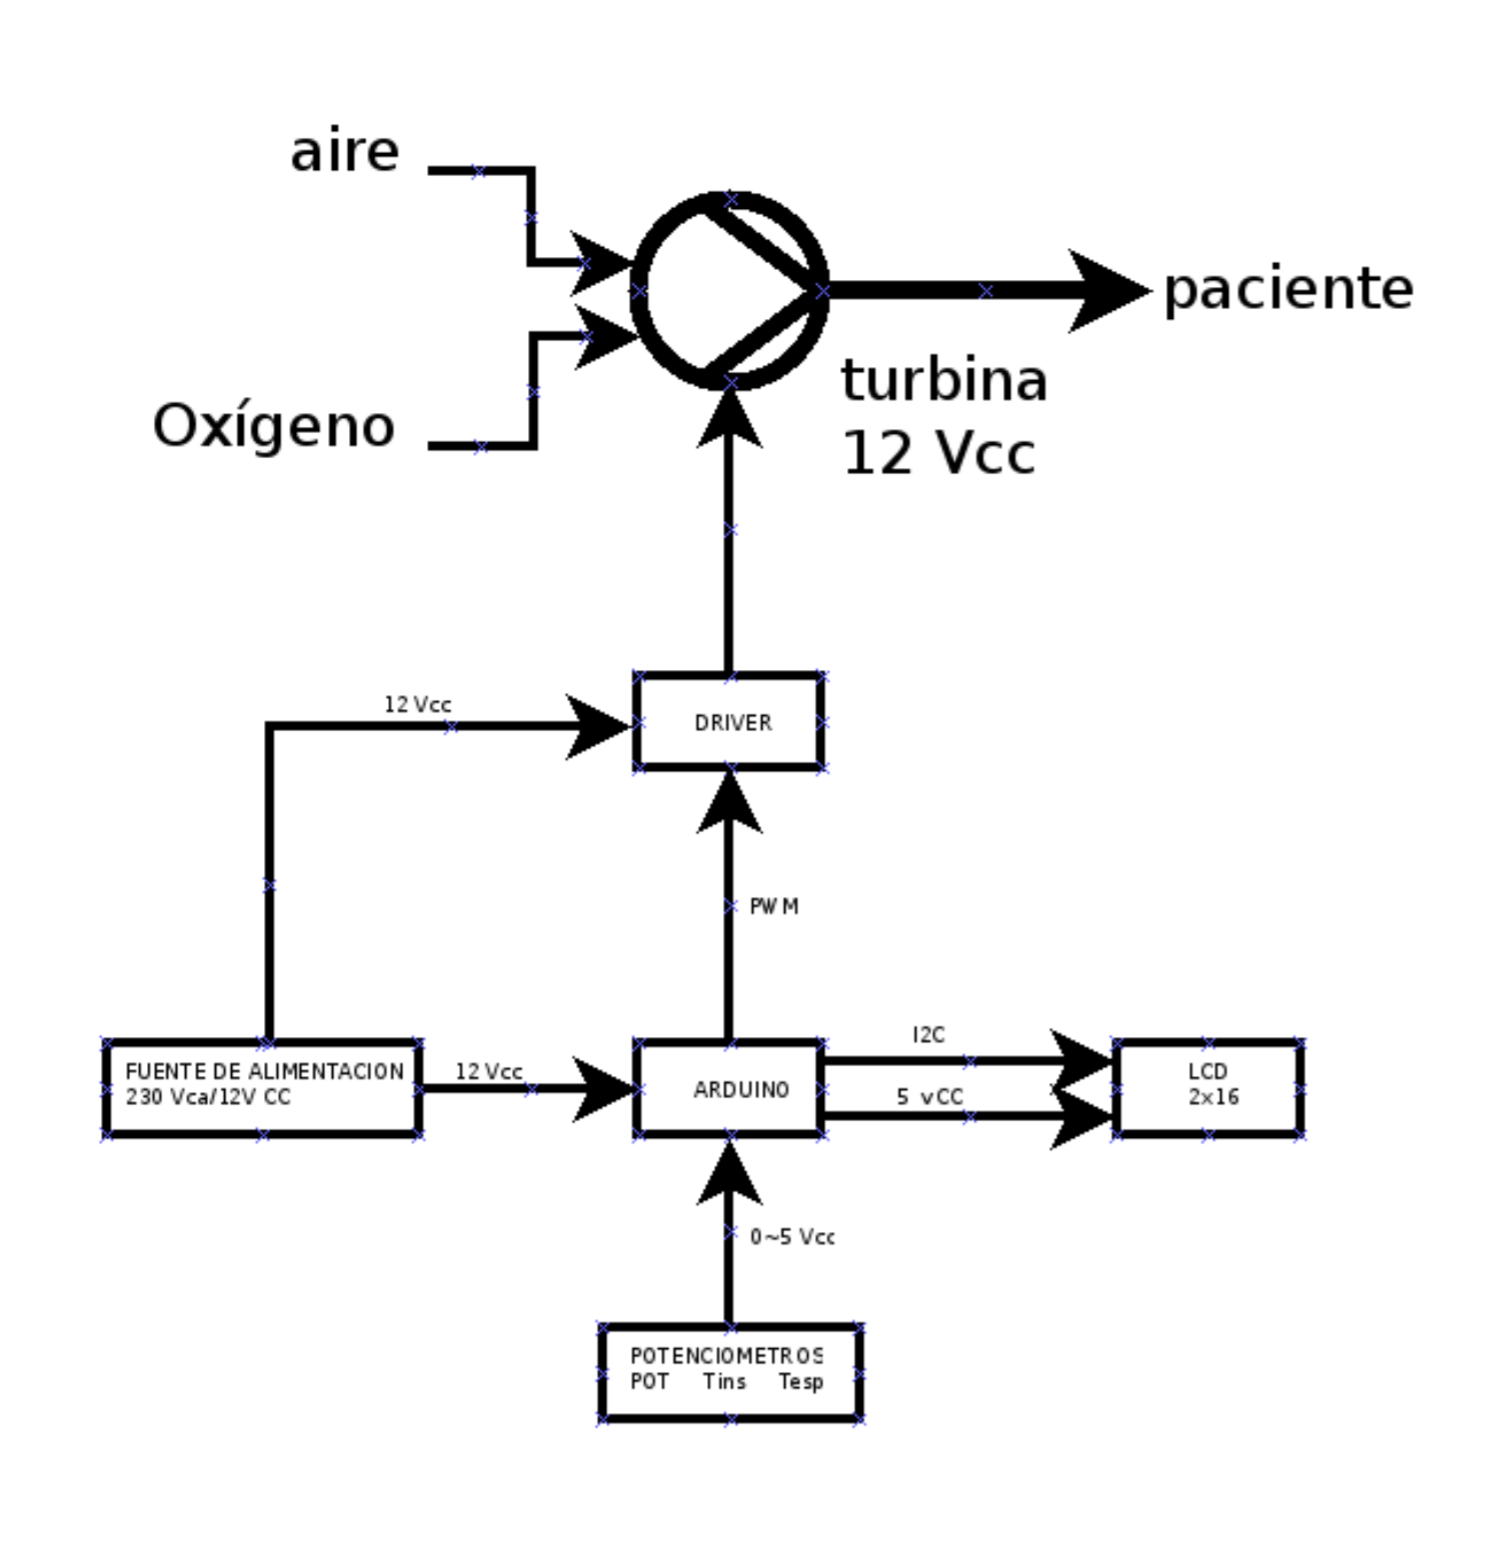
\includegraphics[width=0.4\textwidth]{Img/Bloques.PNG}
        \caption{Block diagram}
    \end{figure}
    The respirator is composed of an air turbine, an electronic board, a power supply and a plastic case.\\
    
    The driving turbine collects air (medical or atmospheric) and oxygen and will drive it to the patient at the rhythm and pressure determined by medical staff. This turbine will be powered from an electronic board, which contains the control system (microcontroller) and a display. The controlling elements are three potentiometers located on the front panel (transparent) and connected to the board by wires. A power 12 \Vcc supplies power to the electronics, and via the electronics, the turbine. The device can be powered by an ambulance battery at 12 \Vcc. The plastic case with a transparent front panel, makes the electrical enclosure isolating the device.
    
    %La turbina impulsora recoge aire (medicinal o atmosférico) y Oxígeno y lo lleva hasta el paciente con el ritmo y presión que determine el personal sanitario. Esa turbina está alimentada desde una placa electrónica que contiene el sistema de control (microcontrolador) y la pantalla. Los elementos de mando son tres potenciómetros situados en la tapa frontal (transparente) y conectados a la placa electrónica por cables. Una fuente de 12 \Vcc alimenta a la electrónica y a través de esta, a la turbina. El equipo puede ser alimentado por la batería de 12 \Vcc de una ambulancia. Por último, una caja de plástico con el frontal transparente constituye la envolvente eléctrica que dota de aislamiento al conjunto.
    
    All the maneuver, parameters and limit values are defined by software.
    %Toda la maniobra y los valores de los parámetros y los valores límite de las variables están definidos por software.
    \begin{figure}
        \centering
        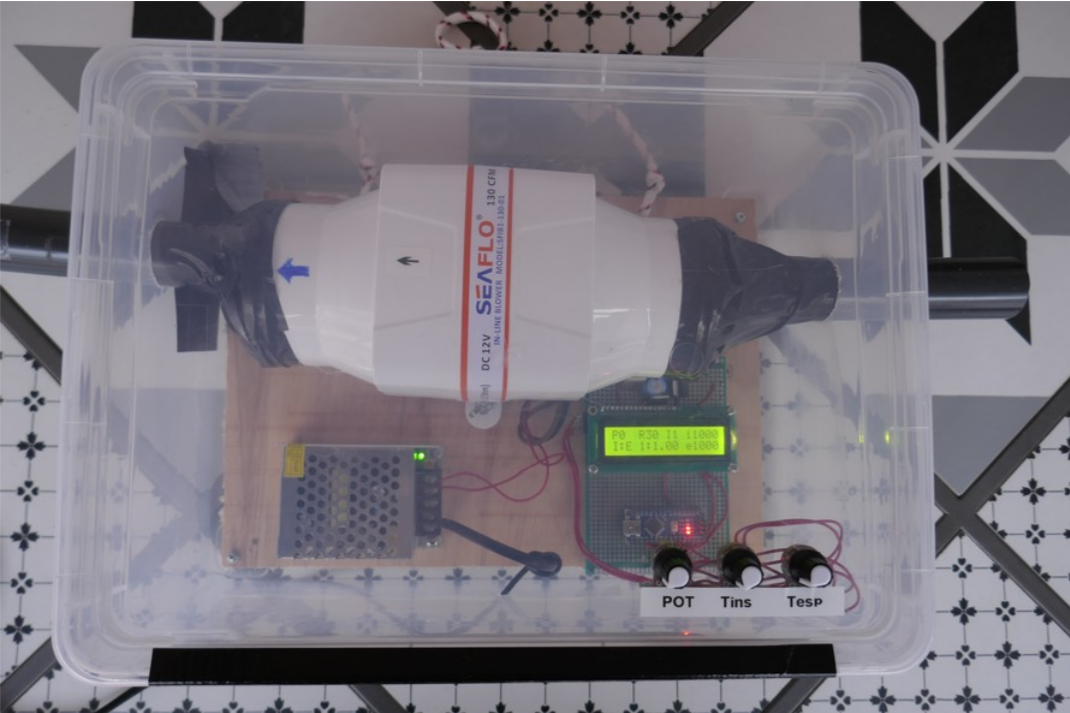
\includegraphics[width=0.4\textwidth]{Img/prototipo-1.PNG}
        \caption{First prototype}
    \end{figure}
    
\subsection{Turbine}
    The electric motor blower at 12\Vcc or 24\Vcc is controlled by a pulse width modulated power transistor. The one used in the prototype comes from the nautic market (it is a bilge ventilator)\\    
    %El soplador con motor eléctrico de 12 \Vcc o de 24 \Vcc está controlado por un transistor de potencia con modulación por anchura de pulso. El usado en el prototipo procede del mercado náutico (es un ventilador de sentina).\\
    It must be able to blow 600ml (excepcionally 800ml) at a preassure up to 70cmH\textsubscript{2}O
    %Debe ser capaz de soplar 600 ml (800 ml excepcionalmente) a una presión de hasta 70 cmH\textsubscript{2}0\\
    If an alternating current blower was needed, would force to redesign both the hardware and the software (can be done fast).
    %Si hiciera falta usar un ventilador de corriente alterna a 230\Vca, debería rediseñarse tanto el hardware como el software (puede hacerse muy rápidamente).

\subsection{Electronic Board}
    The electronic board incorporates the following elements:
    %La tarjeta electrónica incorpora los siguientes elementos:
    \begin{itemize}
        \item Current stabilizer  %Estabilizador de tensión
        \item Display %Pantalla
        \item Computer %Ordenador
        \item Motor signal amplifyer  %Amplificador de salida al motor
    \end{itemize}
    The current stabilizer objective is to supply at 5 \Vcc all the electronic active components. It is composed by an integrated regulator type \textit{7805} in a box \textit{TO220} without radiator, with filtered capacitors an input and output.\\
    %   El estabilizador de tensión tiene por objeto alimentar a 5 \Vcc a todos los elementos electrónicos activos. Está compuesto por un regulador integrado tipo \textit{7805} en caja \textit{TO220} sin radiador, con condensadores de filtro en la entrada y en la salida.\\

    The display is a retro iluminated, two lines, 16 character display. It is connected to the computer via an \textit{I2C} serial bus.\\
    %La pantalla es del tipo LCD retroiluminada de dos filas de 16 caracteres, conectada al ordenador mediante un bus serie tipo \textit{I2C}.\\
    
    The computer is an \textit{Arduino Nano} build with a micro controller ATMEL \textit{ATmega328}. The program is design in the \textit{Arduino} environment and loads in the computer flash memory via USB interface. It is easy and cheap to obtain at around 3€.\\
    %El ordenador es un modelo \textit{Arduino Nano} construido desde un microcontrolador ATMTEL \textit{ATmega328}. El     programa está desarrollado en el entorno \textit{Arduino} y se carga en memoria flash del ordenador por el interface USB. Se puede conseguir fácilmente en el mercado y es muy barato (desde 3€).\\
    
    The motor output amplifier is built by a middle power NPN Darlington transistor type \textit{TIP120}. It is design to be able to use FET-MOS transistos, encapsulated with the case design (TO220), like the \textit{IRF3710}.\\
    %El amplificador de salida del motor está constituido por un transistor de media potencia NPN en montaje Darlington tipo \textit{TIP120} y está diseñado para poder usar transistores FET-MOS encapsulados en el mismo tipo de caja (TO220), como el \textit{IRF3710}.
    
\subsection{Potentiometers}
    The control elements consist of three linear potentiometers mounted over a printed circuit board. These control maximum power, inhaling time and exhale time. The three are mounted over the front pannel to make them accessible.\\
    %Tres potenciómetros lineales montados sobre un pequeño circuito impreso constituyen los elementos de control sobre potencia máxima de la turbina, tiempo de inspiración y tiempo de espiración. Los tres están montados sobre la tapa frontal para hacerlos accesibles.\\
    
    Limit values, both minimum and maximum for each potentimeter are software defined, as the magnitudes controlled by each one. Making modifications easy.
    %Los valores límite máximo y mínimo de cada potenciómetro están definidos por software, así como las propias magnitudes que controlan, con lo que pueden modificarse fácilmente.

\subsection{Case}
    The set is mounted over a mounting plate, screwed over the bottom of the case. This must provide both structural sturdiness and mechanical and electrical shielding needed in a medical enviroment. It must be posible to be cleaned and disinfected while working.\\ 
    %Todo el conjunto se monta sobre una placa de montaje que a su vez se atornilla sobre el fondo de la caja. Esta debe proveer, no solo la robustez estructural del conjunto, sino también la protección mecánica y eléctrica necesaria en un entorno hospitalario. De ser capaz de ser limpiada y desinfectada en funcionamiento.\\
    
    Final working products will be comercial plastic enclosures with the propper characteristics and a transparent pannel.
    %Los ejemplares de producción final serán envolventes plásticas comerciales de las característica adecuadas con tapa transparente.